Die Zertifizierungstelle wird mittels eines Personal Computer (PC) simuliert. Die Zertifikate und Schlüssel werden vom PC mittels \textit{mbedTLS} generiert und beim "`Flashen"' des jeweiligen Programmes auf die Mikrocontroller als Dateien übertragen. Jedoch werden sie nicht in Keystores gespeichert. Die Zertifkate werden nach dem Standard X.509 erstellt und die Schlüssel mittels des RSA-Verfahrens generiert. In Abb. \ref{fig: impl certs keys} wird gezeigt, wie sie erstellt bzw. generiert werden.
\begin{figure}[H]
    \centering
    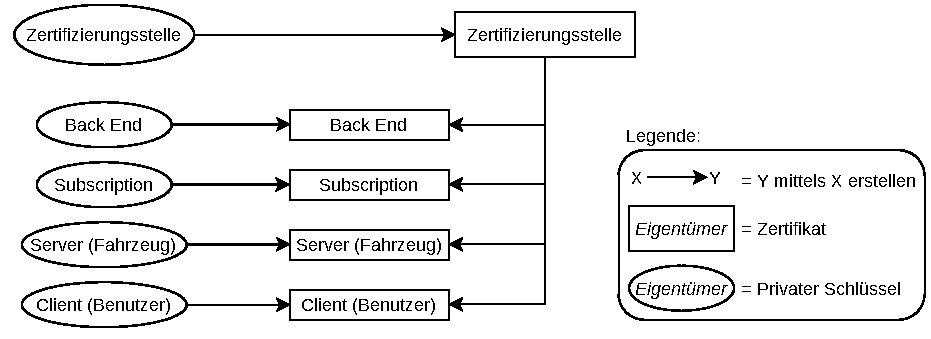
\includegraphics[width=0.9\textwidth]{graphics/impl_keys_certs.pdf}
    \caption[Generierung der Schlüssel und Erstellung der Zertifikate]{Generierung der Schlüssel und Erstellung der Zertifikate}
    \label{fig: impl certs keys}
\end{figure}
Zuerst wird ein 4096 Bit langer privater Schlüssel für die Zertifizierungsstelle generiert. Danach wird das zugehörige Root-Zertifikat mit diesem Schlüssel erstellt. Dabei wird angegeben, dass es ein selbstunterzeichnetes Zertifikat ist und für eine Zertifizierungsstelle ausgestellt wird. Der Name des Ausstellers ist in diesem Fall auch der Name des Eigentümers. Alle weiteren privaten Schlüssel sind ebenfalls 4096 Bit lang. Wurden sie generiert, wird mit jedem privaten Schlüssel genau ein Zertifikat erstellt, dessen Ausstellerzertifikat das Root-Zertifikat ist.
\\\\
Nun liegen alle Zertifikate und Schlüssel vor und werden beim "`Flashen"' des jeweiligen Programmes folgendermaßen auf die beiden Mikrocontroller übertragen:
\begin{itemize}
    \item Server-Mikrocontroller (Fahrzeug):
    \begin{itemize}
        \item privater Server-Schlüssel (Fahrzeug)
        \item Server-Zertifikat (Fahrzeug)
        \item Root-Zertifikat
    \end{itemize}
    \item Client-Mikrocontroller (stellvertretend für die App):
    \begin{itemize}
        \item privater Client-Schlüssel (App)
        \item Client-Zertifikat (App)
        \item privater Subscription-Schlüssel
        \item Subscription-Zertifikat
        \item Root-Zertifikat
    \end{itemize}
\end{itemize}
Der Client erhält zusätzlich den Schlüssel und das Zertifikat zum Erstellen der Subscriptions, um damit das Back End zu simulieren (siehe Sektion \ref{sec: impl prototyp back end}).